% !TEX program = xelatex

% \documentclass[usenames,xcolor=svgnames,11pt,sans,aspectratio=169,handout]{beamer}
\documentclass[usenames,xcolor=svgnames,11pt,sans,aspectratio=169]{beamer}
\usetheme{Madrid}
\colorlet{theme}{DarkGreen}
\usecolortheme[named=theme]{structure}
\newcommand{\key}[1]{{\color{theme} #1}}

\usepackage{xeCJK}
\setCJKmainfont{SimHei}
\usepackage[T1]{fontenc}
\usepackage{zi4}

\usepackage{amsmath}
\usepackage{amssymb}
\usepackage[inference]{semantic}
\usepackage{mathpartir}
\usepackage{empheq}
\newcommand{\boxedeq}[1]{\begin{empheq}[box=\fbox]{align*}#1\end{empheq}}

\usepackage{graphics}
\usepackage{tikz}
\usepackage{hyperref}

\let\t\texttt
\let\le\leqslant
\let\ge\geqslant
\let\disp\displaystyle

% toy lang
\newcommand{\z}{\textsf{zero}}
\newcommand{\s}[1]{\textsf{succ}~#1}
\newcommand{\plus}[2]{\textsf{plus}~#1~#2}
\newcommand{\nil}{\textsf{nil}}
\newcommand{\cons}[2]{\textsf{cons}~#1~#2}
\newcommand{\len}[1]{\textsf{len}~#1}
\newcommand{\idx}[2]{\textsf{idx}~#1~#2}
\newcommand{\sgt}[1]{\textsf{sgt}~#1}

\newcommand{\num}[1]{\key{\textsf{num}}~#1}
\newcommand{\lst}[1]{\key{\textsf{lst}}~#1}
\newcommand{\val}[1]{\key{\textsf{value}}~#1}

\newcommand{\Nat}{\key{\textsf{Nat}}}
\newcommand{\List}{\key{\textsf{List}}}

\begin{document}

% credits
\title{Code is Cheap, Show Me the Proof}
\subtitle{A Rush Introduction to Coq}
\author{Paul Zhu}
\date{\today}

% contents
\AtBeginSection[]
{
    \begin{frame}{Contents}
    	\tableofcontents[currentsection]
	\end{frame}
}

\AtBeginSubsection[]
{
    \begin{frame}{Contents}
    	\tableofcontents[currentsubsection]
	\end{frame}
}

% titlepage
\begin{frame}
    \titlepage
\end{frame}

\begin{frame}{Today}
    \tableofcontents
\end{frame}

\section{Introduction}

\begin{frame}{Installation}
  \begin{itemize}
    \item Home page: \url{https://coq.inria.fr}
    \item Github repo: \url{https://github.com/coq/coq}
    \item CoqIDE: \url{https://github.com/coq/coq/releases}
    \item From OPAM: \url{https://coq.inria.fr/opam-using.html}
    \item From source: \url{https://github.com/coq/coq/blob/master/INSTALL}
    \item Document: \url{https://coq.inria.fr/refman/index.html}
  \end{itemize}

  \vspace{.5cm}
  \begin{columns}
    \begin{column}{.2\textwidth}
      \begin{center}
        
\includegraphics[height=2cm]{fig/barron_logo}
      \end{center}
    \end{column}
    \begin{column}{.8\textwidth}
      Coq is a \key{formal proof} management system.
      It provides a formal language to write mathematical definitions,
      executable algorithms and theorems together with an environment for \key{semi-interactive} development of \key{machine-checked} proofs.
    \end{column}
  \end{columns}
\end{frame}

\begin{frame}{Applications}
  \begin{quote}
    Un des points les plus remarquables de Coq est la possibilité de synthétiser des programmes certifiés à partir de preuves,
    et, depuis peu, des modules certifiés.

    \rightline{-- Le Coq'Art (V8)}
  \end{quote}
  \begin{itemize}
    \item<1-> Verified C compiler: \href{http://compcert.inria.fr}{CompCert}
    \item<2-> Verified operating system: \href{http://flint.cs.yale.edu/certikos/index.html}{CertiKOS}
    \item<3-> Four color theorem
    \item<4-> \href{http://r6.ca/Goedel/goedel1.html}{Gödel's incompleteness theorem}
    \item<5-> \href{https://github.com/HoTT/HoTT/}{Homotopy type theory}
    \item<6-> \href{https://iris-project.org}{Iris: a higher-order concurrent separation logic framework}
    \item<7-> \href{https://github.com/coq-contribs/coq-in-coq}{Coq in Coq}
  \end{itemize}
\end{frame}

\begin{frame}{Coq Workshops}
  \begin{itemize}
    \item \href{https://coq-workshop.gitlab.io}{Coq Workshops} (generally colocated with ITP)
    \item \href{https://coq.inria.fr/coqpl.html}{CoqPL} (colocated with POPL)
    \item \href{https://deepspec.org/page/Event/}{DeepSpec} (colocated with PLDI since 2017)
  \end{itemize}
\end{frame}

\begin{frame}{Why Formal Proof?}
  \linespread{1.8}
  \begin{quote}
    If debugging is the process of removing bugs, then programming must be the process of putting them in.

    \rightline{-- Edsger W. Dijkstra}
  \end{quote}
\end{frame}

\begin{frame}{Why Formal Proof?}
  \linespread{1.8}
  \begin{quote}
    \begin{center}
      西江月·数学证明题
    \end{center}
    
    即得易见平凡,仿照上例显然。留作习题答案略,读者自证不难。
    
    反之亦然同理,推论自然成立。略去过程QED,由上可知证毕。

    \rightline{-- 佚名}
  \end{quote}
\end{frame}

\begin{frame}{Gallina}
  A concise primitive language for expressing logical theories, using keywords:
  \begin{itemize}
    \item \t{Definition}
    \item \t{Inductive} / \t{CoInductive}
    \item \t{Fixpoint} / \t{CoFixpoint}
    \item \t{Axiom}
    \item \t{Theorem} / \t{Lemma} / \t{Fact} / \t{Example}
    \item etc.
  \end{itemize}
\end{frame}

\begin{frame}{Tactic Language}
  An extensive (and extensible) language of tactics to write proof scripts, useful commands:
  \begin{itemize}
    \item \t{intros}, \t{rewrite}, \t{simpl}, \t{reflexivity}
    \item \t{induction}, \t{destruct}
    \item \t{inversion}
    \item \t{split}, \t{left}, \t{right}, \t{exists}
    \item \t{apply}, \t{exact}
    \item \t{auto}
    \item etc.
  \end{itemize}
  and a ``meta language'' to write macros for tactics, supporting pattern matching, composing,
  repeating, etc.
\end{frame}

\begin{frame}{Vernacular}
  An extensive language of commands to manage the proof development environment:
  \begin{itemize}
    \item notations,
    \item implicit arguments, and
    \item type classes.
  \end{itemize}
\end{frame}

\begin{frame}{Learning Coq}
  Books:
  \begin{itemize}
    \item \href{https://softwarefoundations.cis.upenn.edu}{Software Foundations}
    \item \href{https://math-comp.github.io/mcb/book.pdf}{Mathematical Components}
    \item \href{https://www.labri.fr/perso/casteran/CoqArt/coqartF.pdf}{Le Coq'Art (V8)}
  \end{itemize}

  Courses:
  \begin{itemize}
    \item \href{https://www.seas.upenn.edu/~cis500/current/index.html}{CIS 500} instructed by Benjamin Pierce at University of Pennsylvania
    \item See \href{https://github.com/coq/coq/wiki/CoqInTheClassroom}{this page} for more
  \end{itemize}
\end{frame}

\section{Tutorials}

\subsection{Logic \& Curry-Howard Correspondence}

\begin{frame}{Types as Propositions}
  \boxedeq{a : A \iff a~\text{is a proof of}~A}

  \begin{center}
    \begin{tabular}{cc}
      Types & Propositions \\
      \hline
      $0$ & $\bot$ \\
      $1$ & $\top$ \\
      $A \times B$ & $A \land B$ \\
      $A + B$ & $A \lor B$ \\
      $A \to B$ & $A \to B$ \\
      $\Pi_{x: A}~B(x)$ & $\forall x \in A, B(x)$ \\
      $\Sigma_{x: A}~B(x)$ & $\exists x \in A, B(x)$ \\
      $\text{Id}_A(a, b)$ & $a = b$
    \end{tabular}
  \end{center}
\end{frame}

\subsection{Functional Programming \& Functional Correctness}

\begin{frame}{List}
  \centering
  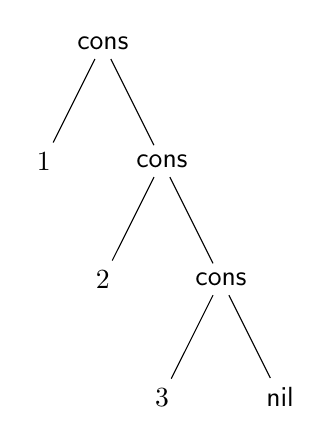
\begin{tikzpicture}
    \node {\textsf{cons}}
        child {
          node {$1$}
        }
        child {
          node {\textsf{cons}}
          child {
            node {$2$}
          }
          child {
            node {\textsf{cons}}
            child {
              node {$3$}
            }
            child {
              node {\textsf{nil}}
            }
          }
        }
    ;
  \end{tikzpicture}

  $[1,2,3]$
\end{frame}

\subsection{Formalizing Your Theory}

\begin{frame}{ToyLang: Syntax}
  \begin{align*}
    \text{Term}~t &::= \z \\
      &\mid \s{t_1} \\
      &\mid \plus{t_1}{t_2} \\
      &\mid \nil \\
      &\mid \cons{t_1}{t_2} \\
      &\mid \len{t_1} \\
      &\mid \idx{t_1}{t_2} \\
      &\mid \sgt{t_1}
  \end{align*}
\end{frame}

\begin{frame}{ToyLang: Value}
  \begin{mathpar}
    \inference[num-zero]{}{\num\z}
    \and \inference[num-succ]{\num{n}}{\num{(\s{n}})} \\
    \and \inference[lst-nil]{}{\lst\nil}
    \and \inference[lst-cons]{\num{n} & \lst{n}}{\lst{(\cons{n}{l}})} \\
    \and \val{t} := \num{t} \lor \lst{t}
  \end{mathpar}
\end{frame}

\begin{frame}{ToyLang: Small-Step}
  \boxedeq{t \to t'}
  \begin{mathpar}
    \inference[ST-succ]{t \to t'}{\s{t} \to \s{t'}} \\
    \and \inference[ST-plus-zero]{\num{n}}{\plus{\z}{n} \to n}
    \and \inference[ST-plus-succ]{\num{n_1} & \num{n_2}}{\plus{(\s{n_1})}{n_2} \to \s{(\plus{n_1}{n_2}})}
    \and \inference[ST-plus-1]{t_1 \to t_1'}{\plus{t_1}{t_2} \to \plus{t_1'}{t_2}}
    \and \inference[ST-plus-2]{\num{t_1} & t_2 \to t_2'}{\plus{t_1}{t_2} \to \plus{t_1}{t_2'}} \\
    \and \cdots
  \end{mathpar}
\end{frame}

\begin{frame}{ToyLang: Typing}
  $$\text{Type}~T ::= \Nat \mid \List$$

  \boxedeq{\vdash t : T}
  \begin{mathpar}
    \inference[T-zero]{}{\vdash \z : \Nat}
    \and \inference[T-succ]{\vdash t : \Nat}{\vdash \s{t} : \Nat}
    \and \inference[T-plus]{\vdash t_1 : \Nat & \vdash t_2 : \Nat}{\vdash \plus{t_1}{t_2} : \Nat} \\
    \and \inference[T-nil]{}{\vdash \nil : \List}
    \and \inference[T-cons]{\vdash t_1 : \Nat & \vdash t_2 : \List}{\vdash \cons{t_1}{t_2} : \List} \\
    \and \cdots
  \end{mathpar}
\end{frame}

\section{Summary}

\begin{frame}{Coq CANNOT...}
  \begin{itemize}
    \item<1-> prove everything automatically
    \item<2-> accept any function (\t{Fixpoint}) that actually terminates
    \item<3-> support classical logic directly (however, you may add axioms)
  \end{itemize}
\end{frame}

\begin{frame}{Beyond Coq}
  \begin{itemize}
    \item \href{https://isabelle.in.tum.de}{Isabelle/HOL} (set theory, classical logic)
    \item \href{http://pvs.csl.sri.com}{PVS} (classical logic, refinement types)
    \item \href{https://github.com/agda/agda}{Agda} (CuTT)
    \item \href{https://www.idris-lang.org}{Idris} (type-driven development)
    \item \href{https://leanprover.github.io}{Lean} (CIC-like)
    \item \href{https://arend-lang.github.io}{Arend} (HoTT)
  \end{itemize}
\end{frame}

\begin{frame}{Beyond Proof Assistant}
  \begin{itemize}
    \item Solver-aided programming languages:
    \href{https://www.rise4fun.com/Dafny}{Dafny},
    \href{https://emina.github.io/rosette/}{Rosette}
    \item Software model checking framework: BLAST,
    \href{https://cpachecker.sosy-lab.org}{CPAChecker},
    \href{https://monteverdi.informatik.uni-freiburg.de/tomcat/Website/?ui=tool&tool=automizer}{Ultimate Automizer},
    \href{https://www.cprover.org/cbmc/}{CBMC}
    \item Modeling languages:
    \href{http://nusmv.fbk.eu}{NuSMV},
    \href{http://spinroot.com/spin/whatispin.html}{Spin},
    \href{https://lamport.azurewebsites.net/tla/tla.html}{TLA+},
    \href{https://www.ansys.com/products/embedded-software/ansys-scade-test}{SCADE},
    \href{https://www.prismmodelchecker.org}{PRISM}
  \end{itemize}
\end{frame}

\end{document}
